\subsection{Đề 2}
\Opensolutionfile{ans}[ans/ans-0-B15]
\caulc
\begin{ex}%[2D1N1-1]
	Các khoảng đồng biến của hàm số $y=x^4-8x^2-4$ là
	\choice
		{$(-\infty;-2)$ và $(2;+\infty)$}
		{$(-2;0)$ và $(0;+\infty)$}
		{$(-\infty;-2)$ và $(0;2)$}
		{\True $(-2;0)$ và $(2;+\infty)$}
		\loigiai{Ta có tập xác định của hàm số là $\mathscr{D}=\mathbb{R}$ và $y'=4x^3-16x$ nên $y'=0\Leftrightarrow 
			\hoac{&x=0\\
				&x=-2\\
				&x=2.}$ \\
			Khi đó $y'\ge 0\Leftrightarrow 4x^3-16x\ge 0\Leftrightarrow \hoac{&x\ge 0\\
			&-2\le x\le 0.}$ \\
		Vậy hàm số đồng biến trên các khoảng $(-2;0)$ và $(2;+\infty)$.
		}
\end{ex}

\begin{ex}%[2D1N1-1]
	Hàm số $y=x^4-2x^2+1$ nghịch biến trên các khoảng nào sau đây?
	\choice
		{\True $(-\infty;-1)$ và $(0;1)$}
		{$(-\infty;-1)$ và $(0;+\infty)$}
		{$(-\infty;0)$ và $(1;+\infty)$}
		{$(-1;0)$ và $(1;+\infty)$}
	\loigiai{Ta có $y'=4x^3-4x=0\Leftrightarrow \hoac{&x=0\\
			&x=-1\\
			&x=1.\\
		}$ \\
		Bảng biến thiên
		\begin{center}
			\begin{tikzpicture}
				\tkzTabInit[nocadre = false,lgt = 1,espcl = 2]
				{  $x$  /1,  $y'$  /1,  $y$  /2}{  $-\infty$  ,$-1$, $0$, $1$,  $+\infty$  }
				\tkzTabLine{,-,  $0$ , +, $0$ ,-, $0$, +}
				\tkzTabVar{+/  $+\infty$  ,-/  $0$  , +/ $1$, -/ $0$, +/ $+\infty$  }
			\end{tikzpicture}
		\end{center}
		Vậy hàm số nghịch biến trên các khoảng
		$(-\infty;-1)$ và $( 0;1)$.}
\end{ex}

\begin{ex}%[2D1N1-1]
	Cho hàm số $y=\dfrac{x+1}{x-3}$. Trong các mệnh đề sau, mệnh đề nào \textbf{sai}?
	\choice
		{Hàm số nghịch biến trên từng khoảng xác định của nó}
		{\True Hàm số nghịch biến trên tập xác định của nó}
		{Hàm số nghịch biến trên khoảng $(3;+\infty)$}
		{Hàm số nghịch biến trên khoảng $(-\infty; 3)$}
	\loigiai{Hàm số đã cho có tập xác định gồm hai khoảng $(-\infty; 3)$ và $(3;+\infty)$ rời nhau nên khẳng định hàm số nghịch biến trên tập xác định là sai.}
\end{ex}

\begin{ex}%[2D1N1-1]
	Cho hàm số $y=\dfrac{1}{3}x^3-\dfrac{1}{2}x^2-12x-1$. Mệnh đề nào sau đây đúng?
	\choice
		{Hàm số nghịch biến trên khoảng $(-3;+\infty)$}
		{Hàm số đồng biến trên khoảng $(-\infty;4)$}
		{Hàm số đồng biến trên khoảng $(-3;4)$}
		{\True Hàm số đồng biến trên khoảng $(4;+\infty)$}
	\loigiai{
		Ta có $y'=x^2-x-12=0\Leftrightarrow \hoac{&x=-3\\
			&x=4.}$ \\
		Bảng xét dấu
		\begin{center}
			\begin{tikzpicture}
				\tkzTabInit[lgt = 2,espcl = 2.5]%
				{$x$ /1, $y'$/1}
				{$-\infty$ ,  $-3$,  $4$,  $+\infty$  }
				\tkzTabLine{ ,+,0,-,0,+,}
			\end{tikzpicture}
		\end{center}
		Dựa vào bảng xét dấu ta thấy hàm số đồng biến trên khoảng $(4;+\infty)$.
		}
\end{ex}


\begin{ex}%[2D1H1-1]
	Hàm số nào sau đây \textbf{không} đồng biến trên $(-\infty;+\infty)$ 
	\choice
		{$y=x^5+x^3-1$}
		{$y=x^3+2$}
		{\True $y=\dfrac{x-1}{x+2}$}
		{$y=x+1$}
	\loigiai{
		Ta có $y=\dfrac{x-1}{x+2}\Rightarrow y'=\dfrac{3}{{(x+2)}^2} > 0,\forall x\ne-2$. \\
		Do đó hàm số đồng biến trên các khoảng $(-\infty;2)$ và $(2;+\infty)$.}
\end{ex}

 
\begin{ex}%[2D1H1-1]
	Cho hàm số $y=x-2\sqrt{x}$. Mệnh đề nào sau đây đúng?
	\choice
		{Hàm số nghịch biến trên khoảng $(1;+\infty)$}
		{\True Hàm số đồng biến trên khoảng $(2;+\infty)$}
		{Hàm số đồng biến trên khoảng $(0;+\infty)$}
		{Hàm số nghịch biến trên khoảng $(-\infty;1)$}
	\loigiai{
		Tập xác định $\mathscr{D}=[0;+\infty)$. \\
		Ta có $y'=1-\dfrac{1}{\sqrt{x}}=\dfrac{\sqrt{x}-1}{\sqrt{x}}$;
		$y'=0\Leftrightarrow \sqrt{x}=1\Leftrightarrow x=1$.\\
		Bảng biến thiên
		\begin{center}
			\begin{tikzpicture}
				\tkzTabInit[lgt = 1,espcl = 2.5]%nocadre
				{  $x$  /.7,  $y'$  /.7,  $y$  /2}
				{  $0$  ,  $1$  ,  $+\infty$  }
				\tkzTabLine{,-,  $0$  ,+,}
				\tkzTabVar{+/ $0$  ,-/  $-1$  ,+/  $+\infty$  }
			\end{tikzpicture}
		\end{center}
		Từ bảng biến thiên suy ra $y' < 0,\forall x\in (0;1)$ và $y' > 0,\forall x\in (1;+\infty)$.\\
		Vậy hàm số đồng biến trên khoảng $(1;+\infty)$ suy ra hàm số đồng biến trên khoảng $(2;+\infty)$.
		}
\end{ex} 

\begin{ex}%[2D1H1-3]
	Cho hàm số $y=f(x)$ xác định liên tục và liên tục trên $\mathbb{R}$ và có bảng biến thiên như sau
	\begin{center}
		\begin{tikzpicture}
			\tkzTabInit[nocadre = false,lgt = 1,espcl =3.5]
			{$x$  /1,  $y'$  /1,  $y$  /2}{  $-\infty$  ,  $2$  ,  $+\infty$}
			\tkzTabLine{,-,  $0$  ,+,}
			\tkzTabVar{+/  $+\infty$, -/$0$, +/  $+\infty$  }
		\end{tikzpicture}
	\end{center}
		Khẳng định nào sau đây đúng?
		\choice
			{Hàm số có $2$ cực trị}
			{Hàm số có giá trị cực đại bằng $2$}
			{\True Hàm số có giá trị cực tiểu bằng $0$}
			{Hàm số có giá trị cực đại tại $x=0$}
		\loigiai{Dựa vào bảng biến thiên, ta thấy hàm số đạt cực tiểu tại $x=2$ và $y=0$. Do đó, giá trị cực tiểu của hàm số bằng $0$.}
\end{ex}

\begin{ex}%[2D1H1-3]
	Cho hàm số $y=f(x)$ có bảng biến thiên như sau.
	Mệnh đề nào dưới đây là \textbf{sai?}
	\begin{center}
		\begin{tikzpicture}
					\tkzTabInit[nocadre = false,lgt = 1,espcl = 3]
					{  $x$  /1,  $y'$  /1,  $y$  /2}{  $-\infty$  , $0$,  $2$  ,  $+\infty$  }
					\tkzTabLine{ ,+, $0$, -,  $0$  ,+,}
					\tkzTabVar{-/  $-\infty$ ,+/  $3$  ,-/  $0$  , +/  $+\infty$  }
		\end{tikzpicture}
	\end{center}
		\choice
			{\True Hàm số \textbf{không} đạt cực tiểu tại điểm $x=2$}
			{Hàm số đạt cực đại tại điểm $x=0$}
			{Giá trị cực đại của hàm số là $y=3$}
			{Giá trị cực tiểu của hàm số là $y=0$}
		\loigiai{Hàm số đạt cực tiểu tại điểm $x=2$.}
\end{ex}

\begin{ex}%[2D1H1-3]
	Cho hàm số $y=f(x)$ có bảng biến thiên như sau
	\begin{center}
		\begin{tikzpicture}
					\tkzTabInit[nocadre = false,lgt = 1,espcl = 3]
					{  $x$  /1,  $y'$  /1,  $y$  /2}{  $-\infty$  , $0$,  $2$  ,  $+\infty$  }
					\tkzTabLine{ ,+, $0$, -,  $0$  ,+,}
					\tkzTabVar{-/  $-\infty$ ,+/  $3$  ,-/  $0$  , +/  $+\infty$  }
		\end{tikzpicture}
	\end{center}
		Tìm giá trị cực đại $y_{\text{CĐ}}$ và giá trị cực tiểu $y_{\text{CT}}$ của hàm số đã cho.
		\choice
			{$y_{\text{CĐ}}=3$ và $y_{\text{CT}}=2$}
			{$y_{\text{CĐ}}=2$ và $y_{\text{CT}}=0$}
			{$y_{\text{CĐ}}=3$ và $y_{\text{CT}}=3$}
			{\True $y_{\text{CĐ}}=3$ và $y_{\text{CT}}=0$}
		\loigiai{
			Dựa vào bảng biến thiên ta có $y_{\text{CĐ}}=3$ và $y_{\text{CT}}=0$.
			}
\end{ex}

\begin{ex}%[2D1V1-1]
	Tìm $m$ để hàm số $y=x^3+mx^2+(1-2m)x+m-3$ đồng biến trên khoảng $(-3;0)$.
	\choice
		{$m \ge 2\sqrt{3}+3$}
		{\True $m\le 2\sqrt{3}-3$}
		{$m \ge 6-\sqrt{42}$}
		{$m \le 6+\sqrt{42}$}
	\loigiai{
		Hàm số $y=x^3+mx^2+(1-2m)x+m-3$ xác định với mọi $x\in\mathbb{R}$ và \[y'=3x^2+2mx+(1-2m).\]
		Hàm số đồng biến trên khoảng $(-3;0)$ khi và chỉ khi $y ' \ge 0$ với mọi $x\in (-3;0)$. \\
		 $3x^2+2mx+1-2m \ge 0, \ \forall x \in (-3;0) \Leftrightarrow \dfrac{3x^2+1}{2-2x} \ge m, \ \forall x \in (-3;0)$. \hfill $(1)$ \\
		Đặt $f(x)=\dfrac{3x^2+1}{2-2x}$, $x\in (-3;0)$. Với mọi $x\in (-3;0)$ ta có $f'(x)=\dfrac{-6x^2+12x+2}{(2x-2)^2}$.\\
		$$ f'(x)=0\Rightarrow-6x^2+12x+2=0 \Leftrightarrow \hoac{& x=\dfrac{3+2\sqrt{3}}{3} \notin (-3;0) \\
			& x=\dfrac{3-2\sqrt{3}}{3} \in (-3;0).} $$
		\begin{center}
			\begin{tikzpicture}
				\tkzTabInit[nocadre = false,lgt = 1.2,espcl = 3.5]
				{$x$  /1.25,  $f'(x)$  /0.7,  $f(x)$  / 3}{  $-3$  ,  $\dfrac{3-2\sqrt{3}}{3}$  ,  $0$}
				\tkzTabLine{,-,  $0$  ,+,}
				\tkzTabVar{+/  $\dfrac{7}{2}$  ,-/  $-3+2\sqrt{3}$  ,+/  $\dfrac{1}{2}$  }
			\end{tikzpicture}
		\end{center}
			Dựa vào bảng biến thiên của $f(x)$ ta có $(1) \Leftrightarrow m \le -3+2\sqrt{3}$.
			}
\end{ex}

\begin{ex}%[2D1V1-1]
	Tất cả các giá trị của tham số $m$ sao cho hàm số $y=-x^3-3mx^2+4m-1$ đồng biến trên khoảng $(0;4)$ là
	\choice
		{$-2\leqslant m < 0$}
		{$m\leqslant-4$}
		{\True $m\leqslant-2$}
		{$m > 0$}
	\loigiai{
		Ta có $y'=-3x^2-6mx$. Cho $y'=0\Leftrightarrow 
		\left[\begin{aligned}
			&x=0\\
			&x=-2m.
		\end{aligned}\right.$\\
		Nếu $m=0$ thì hàm số nghịch biến trên $\mathbb{R}$ (không thỏa mãn yêu cầu bài toán). Từ đó $m\neq 0$. \\
		Giả sử $\{x_1;x_2\}=\{0;-2m\}$, với $m<0$ và $x_1< x_2$. Ta có bảng biến thiên của hàm số
		\begin{center}
			\begin{tikzpicture}
					\tkzTabInit[nocadre = false,lgt = 1,espcl = 3]
					{  $x$  /1,  $y'$  /1,  $y$  /2}{  $-\infty$  ,  $0$, $-2m$ ,  $+\infty$  }
					\tkzTabLine{,+,$0$,-,  $0$  ,+,}
					\tkzTabVar{-/  $-\infty$  ,+/  $-1$ , -/$y(-2m)$  , +/  $+\infty$  }
			\end{tikzpicture}
		\end{center}
			Như vậy hàm số nghịch biến trên khoảng $(0;4)$.
			$$ \Leftrightarrow x_1\leqslant 0< 4\leqslant x_2\Leftrightarrow \left\{\begin{aligned}	& x_1=0\\
			&x_2=-2m \geqslant 4\end{aligned}\right. \Leftrightarrow m \leqslant-2. $$}
\end{ex}

\begin{ex}%[2D1V1-1]
	Tìm tất cả các giá trị của tham số $m$ để hàm số $y=-x^3+3x^2+3mx-1$ nghịch biến trên khoảng $(0;+\infty)$.
	\choice
		{$m >-1$}
		{$m\geq-1$}
		{\True $m\leq-1$}
		{$m <-1$}
	\loigiai{
		Ta có $y'=-3x^2+6x+3m$.\\
		Hàm số đã cho nghịch biến trên $(0;+\infty)$ khi và chỉ khi $y'\leq 0, \forall x\in (0;+\infty)$ 
		\begin{align*}
			&\Leftrightarrow-3x^2+6x+3m\leq 0, \forall x\in (0;+\infty)\\
			&\Leftrightarrow m\leq x^2-2x, \forall x\in (0;+\infty)\\
			&\Leftrightarrow m\leq \min\limits_{[0;+\infty)}(x^2-2x)\\
			&\Leftrightarrow m\leq-1.
		\end{align*}}
\end{ex}
\Closesolutionfile{ans}
\indapan{6}{ans/ans-0-B15}

\cauds
\Opensolutionfile{ans}[ans/ans-0-B15-DS]

\begin{ex}%[2D1H2-2]
		Đạo hàm $f'(x)$ của hàm số $y=f(x)$ có đồ thị như hình bên dưới. Xét tính đúng sai của các mệnh đề sau
		\choiceTF
			{Hàm số đạt cực tiểu tại $x=-1$}
			{\True Hàm số đồng biến trên $(-1;2)$ và $(4;5)$}
			{Hàm số nghịch biến trên $(2;4)$}
			{\True Hàm số $f(x+2)$ đạt cực đại tại $x=0$}
		\begin{center}
		\begin{tikzpicture}[scale=0.7, font=\footnotesize, line join=round, line cap=round, >=stealth]
			\def\a{0.125} \def\b{-0.625} \def\c{0.25} \def\d{1} % Hệ số
			\def\xt{-3} \def\xp{6} \def\yt{2.5} \def\yd{-3} % x_trái, x_phải, y_trên, y_dưới (giới hạn)
			\draw[->] (\xt,0)--(\xp,0) node [below]{$x$};
			\draw[->] (0,\yd)--(0,\yt) node [left]{$y$};
			\node at (0,0) [below right]{$O$};
			\clip (\xt+0.1,\yd-1) rectangle (\xp-0.1,\yt-0.1);
			\draw[smooth,samples=200,domain=-2:5] plot(\x,{\a*(\x)^3+\b*(\x)^2+\c*(\x)+\d}) node [below left]{$y=f'(x)$};
			\draw[dashed] (-2,0) node [below left]{$-2$} -- (-2,-3) 
							(5,0) node [below]{$5$} -- (5,2.25);
			\fill (-1,0) circle (1.5pt) node[below right]{$-1$}
					(2,0) circle (1.5pt) node[below left]{$2$}
					(4,0) circle (1.5pt) node[below right]{$4$};
		\end{tikzpicture}
	\end{center}
	\loigiai{
		Từ đồ thị ta thấy $f'(x)=0 \Leftrightarrow \hoac{& x=-1\\ & x=2\\ & x=4.}$\\
		Ta có bảng biến thiên như sau
		\begin{center}
			\begin{tikzpicture}
				\tkzTabInit[nocadre=true,lgt=1.2,espcl=2.5,deltacl=0.6]
				{$x$ /0.6,$f'(x)$ /0.6,$f(x)$ /2}
				{$-2$,$-1$,$2$,$4$,$5$}
				\tkzTabLine{,-,$0$,+,$0$,-,$0$,+,}
				\tkzTabVar{+/,-/,+/,-/,+/}
			\end{tikzpicture}
		\end{center}
		\begin{itemchoice}
			\itemch Hàm số đạt cực tiểu tại $x=-1$, $x=4$.
			\itemch Hàm số đồng biến trên $(-1;2)$ và $(4;5)$.
			\itemch Hàm số nghịch biến trên $(-2;-1)$ và $(2;4)$.
			\itemch Hàm số $f(x)$ đạt cực đại tại $x=2$. Suy ra hàm số $f(x+2)$ đạt cực đại tại $x=0$.
		\end{itemchoice}
	}
\end{ex}

\begin{ex}%[2D1H1-1]
	Cho hàm số $y=f(x)$ xác định trên $\mathbb{R}$ và có bảng biến thiên như hình vẽ.
	\begin{center}
		\begin{tikzpicture}
				\tkzTabInit[lgt = 1.5,espcl = 3]%
				{$x$ /1, $f'(x)$/1}
				{$-\infty$ ,  $-1$,  $1$,  $+\infty$  }
				\tkzTabLine{ ,+,0,-,0,+,}
		\end{tikzpicture}
	\end{center}
	Xét tính đúng, sai của các mệnh đề sau.
	\choiceTF
		{\True Hàm số có $2$ cực trị}
		{\True Hàm số nghịch biến trên khoảng $(-1;1)$}
		{Hàm số đồng biến trên khoảng $(1;+\infty)$}
		{\True Hàm số $f(1-x)$ đồng biến trên khoảng $(-1;1)$}
	\loigiai
		{Dựa vào bảng biến của hàm số $y=f(x)$ ta có
		\begin{itemchoice}
			\itemch Hàm số đạt cực đại tại $x=-1$ và đạt cực tiểu tại $x=1$.
			\itemch Hàm số nghịch biến trên khoảng $(-1;1)$.
			\itemch Hàm số đồng biến trên mỗi khoảng $(-\infty;-1)$, $(1;+\infty)$.
			\itemch Đặt $g(x)=f(1-x)$. Ta có $g'(x)=-f'(1-x)$ nên $g'(x)>0$, $\forall x\in (-1,1)$. Do đó, hàm số $f(1-x)$ đồng biến trên khoảng $(-1;1)$.
		\end{itemchoice}
		}
\end{ex}

\begin{ex}%[2D1H1-1]
	Cho hàm số $y=f(x)$ xác định trên $\mathbb R$ và có đồ thị của hàm số $y=f'(x)$ là đường cong ở hình vẽ dưới. 
	\choiceTF
		{Hàm số $f(x)$ đạt cực đại tại $x=0$}
		{Hàm số $f(x)$ nghịch biến trong khoảng $(0;2)$}
		{\True Hàm số $f(x)$ có $2$ khoảng đồng biến và $2$ khoảng nghịch biến}
		{\True Hàm số $f(x)$ có $3$ điểm cực trị}
		\begin{center}
				\begin{tikzpicture}[scale = 0.7, > = stealth]
						%Vẽ hai trục
						\draw[- > ](-3,0)--(4,0) node[below]{\tiny  $x$  };;
						\draw[- > ](0,-3.5)--(0,3.5) node[left]{\tiny  $y$  };
						\foreach \y/\ytext in {-2/-2,2/2}
						\draw(0,\y) node[left] {\tiny  $\ytext$ };
						\path (2,0) node[above]{\tiny  $2$  };
						\node[below left](0,0){\tiny  $O$  };
						\draw[smooth,samples = 100,domain = -1.1:3.1]
						plot(\x,{(\x)^3-3*(\x)^2+2});
						% Vẽ đường gióng
						\draw[dashed] (0,-2) -- (2,-2) -- (2,0);
						\path (3.25,2.75) node[anchor=east,font=\scriptsize]{$y=f'(x) $};
				\end{tikzpicture}
		\end{center}
	\loigiai{
		\begin{itemchoice}
			\itemch  Tại $x=0$ hàm $f'(x)$ đạt cực đại nhưng $f(x)$ không đạt cực đại.
			\itemch  Trong khoảng $(0;2)$ đạo hàm có khoảng dương và âm nên $f(x)$ không đồng biến.
			\itemch  Hàm số $f'(x)$ có $2$ khoảng âm và $2$ khoảng dương nên hàm số $f(x)$có $2$ khoảng đồng biến và $2$ khoảng nghịch biến.
			\itemch Ta thấy $f'(x)$ đổi dấu $3$ lần nên đồ thị hàm số $y=f(x)$ có ba cực trị.
		\end{itemchoice}
		}
\end{ex}

\begin{ex}%[2D1H1-4]
	 Cho hàm số $y=f(x)$ liên tục trên đoạn $\left[0 ; \dfrac{16}{5}\right]$ thoả mãn\\ 
	 $f'\left(\dfrac{1}{3}\right)=f'(1)=f'\left(\dfrac{5}{2}\right)=0$ và có đồ thị là đường cong như hình dưới. 
	 \begin{center}
	  		\begin{tikzpicture}[line cap=butt,line join=miter,>=stealth,font=\footnotesize,scale=.7]
	 			\tikzset{declare function={xmin=-2;xmax=4;ymin=-3;ymax=3;
	 					f(\x)=32/45*(\x)^4-32/9*(\x)^3+224/45*(\x)^2-32/15*(\x);
	 				},
	 				smooth,samples=250
	 			}
	 			\draw[->] (xmin,0)--(xmax,0) node[shift={(-100:7pt)}]{$ x $};
	 			\draw[->] (0,ymin)--(0,ymax) node[shift={(10:7pt)}]{$ y $};
	 			\fill (0,0) node[shift={(135:10pt)}]{$ O $};
	 			\draw[dashed](1/3,0)node[shift={(90:8pt)}]{$\tfrac{1}{3}$}|-(0,-1/3.5)node[shift={(-150:9pt)}]{$-\tfrac{1}{3}$}
	 			(2.5,0)node[shift={(90:7pt)}]{$\tfrac{5}{2}$}|-(0,-2)node[shift={(180:9pt)}]{$-2$}	(1,0)node[shift={(90:7pt)}]{$1$}
	 			(3.2,0) node[shift={(-90:7pt)},font=\scriptsize]{$\tfrac{16}{5}$} |-(0,{f(3.2)}) node[shift={(180:7pt)}]{$3$};
	 			\clip (xmin,ymin) rectangle (xmax,ymax);
	 			\draw  plot[domain=0:3.2] (\x, {f(\x)});
	 	\end{tikzpicture}
	 \end{center}
	\choiceTF
		{\True $x=1$ là điểm cực đại của hàm số}
		{\True $x=\dfrac{1}{3}$, $x=\dfrac{5}{2}$ là điểm cực tiểu của hàm số}
		{Hàm số đã cho nghịch biến trên $\left(\dfrac{1}{3};1\right)$ và $\left(\dfrac{5}{2};+\infty\right)$}
		{\True Giá trị lớn nhất của hàm số là $3$}
	\loigiai{
		\begin{itemchoice}
			\itemch $x=1$ là điểm cực đại của hàm số.
			\itemch $x=\dfrac{1}{3}$, $x=\dfrac{5}{2}$ là điểm cực tiểu của hàm số.
			\itemch Hàm số đã cho đồng biến trên $\left(\dfrac{1}{3};1\right)$ và $\left(\dfrac{5}{2};+\infty\right)$; nghịch biến trên $\left(-\infty;\dfrac{1}{3}\right)$ và $\left(1;\dfrac{5}{2}\right)$.
			\itemch Giá trị lớn nhất của hàm số đạt tại $x=\dfrac{16}{5}$, bằng $3$.
	\end{itemchoice}}
\end{ex}

\Closesolutionfile{ans}
%\indapan{3}{ans/ans-0-B15-DS}

\Opensolutionfile{ans}[ans/ans-0-B15-KQ]
\caukq

\begin{ex}%[2D1H1-1]
	Hàm số $y=\dfrac{1}{4}x^4-\dfrac{1}{2}x^3$ có bao nhiêu điểm cực trị?
	\shortans{$1$}
	\loigiai{Ta có $y'=x^3-\dfrac{3}{2}x^2=x^2\left(x-\dfrac{3}{2}\right)$ chỉ đổi dấu khi qua điểm $x=\dfrac{3}{2}$ nên hàm số có 1 điểm cực trị.}
\end{ex}


\begin{ex}%[2D1H1-3]
	Cho hàm số $y=\dfrac{mx+2}{2x+m}$, $m$ là tham số thực. Gọi $S$ là tập hợp tất cả các giá trị nguyên của $m$ để hàm số nghịch biến trên khoảng $(0;1)$. Tìm số phần tử của $S$.
	\shortans{$2$}
	\loigiai{$y'=\dfrac{m^2-4}{(2x+m)^2}$.\\
		Hàm số nghịch biến trên khoảng $(0;1)$ khi và chỉ khi
		\[\heva{&m^2-4< 0\\
			&-\dfrac{m}{2}\notin (0;1)}\Leftrightarrow \heva{&-2< m < 2\\
			&\hoac{&m\ge 0\\
			&m\le-2}}\Leftrightarrow 0\le m < 2.\]
		Vậy số phần tử của tập $S$ là $2$.
		}
\end{ex}


\begin{ex}%[2D1V1-1]
	Tìm giá trị của tham số $m$ để hàm số $f(x)=(m^2-3)x-2m\ln{x}$ đạt cực tiểu tại điểm $x_0=1$.
	\shortans{$3$}
	\loigiai{
		Ta có $f'(x)=m^2-3-2m \cdot \dfrac{1}{x}$ và $f''(x)=2m \cdot \dfrac{1}{x^2}$. \\
		Nhận thấy hàm số có đạo hàm tại $x_0=1$.\\
		Do đó, hàm số đạt cực trị tại $x_0=1$ khi và chỉ khi
		\[ f'(1)=0\Leftrightarrow m^2-3-2m=0\Leftrightarrow \hoac{	&m=-1\\
			&m=3.}\]
		Khi $m=-1$ ta thấy $f''(1) < 0$, do đó hàm số đạt cực đại tại $x_0=1$, loại. \\
		Khi $m=3$ ta thấy $f''(1) > 0$, do đó hàm số đạt cực tiểu tại $x_0=1$, nhận.
		}
\end{ex}

\begin{ex}%[2D1V1-1]
	Gọi $A$, $B$ là hai điểm cực trị của đồ thị hàm số $y=x^3-3x^2+4$. Tính diện tích $S$ của tam giác $OAB$ với $O$ là gốc tọa độ.
	\shortans{$4$}
	\loigiai{
		Ta có $y'=3x^2-6x$ và $y'=0\Leftrightarrow x=0$ hoặc $x=2$.\\
		Do đó hai điểm cực trị của đồ thị hàm số là $A(0;4), B(2;0)$.\\
		Diện tích tam giác vuông $OAB$ là $S_{\triangle OAB}=\dfrac{1}{2}OA\cdot OB=4$.
		}
\end{ex}

\begin{ex}%[2D1C1-1]
	Có bao nhiêu giá trị nguyên của tham số $m$ để hàm số $y=\dfrac 1{3} x ^ 3-(m-1) x ^ 2-(m-3) x+2024m$ đồng biến trên các khoảng $(-3;-1)$ và $(0;3)$?
	\shortans{$4$}
	\loigiai{
		Ta có $y'=x^2-2(m-1)x-(m-3)$ với biệt thức $\Delta'=(m-1)^2+m-3=m^2-m-2$.
		Nếu hàm số đã cho đồng biến trên các khoảng $(-3;-1)$ và $(0;3)$ thì
		$y'\geq 0\;\; \forall x\in (-3;-1)\cup (0;3)$. Do tính liên tục của $y'$ ta suy ra
		\[\heva{& y'(-1)\geq 0\\
				& y'(-3)\geq 0\\
				& y'(0)\geq 0\\
				& y'(3)\geq 0}\Leftrightarrow 
			\heva{& m+2\geq 0\\
				& 5m+6\geq 0\\
				& 3-m\geq 0\\
				& 18-7m\geq 0}\Leftrightarrow-\dfrac{6}{5} \leq m\leq \dfrac{18}{7}.
		\]
		Vì $m$ là số nguyên nên $-1\leq m\leq 2$, khi đó $\Delta'=m^2-m-2\leq 0$ suy ra $y'\geq 0\quad \forall x\in \mathbb{R}$.\\
		Vậy có $4$ giá trị nguyên của $m$ thỏa mãn đề bài.}
\end{ex}

\begin{ex}%[2D1C1-1]
	Gọi $(P)$ là parabol qua 3 điểm cực trị của đồ thị hàm số $y=\dfrac{1}{4}x^4-mx^2+m^2$. Tìm tất cả các giá trị thực của tham số $m$ để $(P)$ qua $A(2;24)$.
	\shortans{$6$}
	\loigiai{$y'=x^3-2mx$, $y'=0\Leftrightarrow\hoac{&x=0\\
		&x^2=2m.}$\\
		 Để đồ thị hàm số có ba cực trị thì $m > 0$.\\
			$y'=0\Leftrightarrow\hoac{	&x=0\Rightarrow y=m^2\\
		&x=\pm\sqrt{2m}\Rightarrow y=0.}$\\
		Vậy ba điểm cực trị của đồ thị hàm số là $A(0;m^2)$, $B(\sqrt{2m};0)$, $C(-\sqrt{2m};0)$.\\
		Gọi $(P)\colon y=ax^2+bx+c$ là parabol qua ba cực trị của đồ thị hàm số.\\
		$\Rightarrow\heva{&c=m^2\\
			&2ma+b\sqrt{2m}+c=0\\
			&2ma-b\sqrt{2m}+c=0}\Leftrightarrow\heva{&c=m^2\\
			&a=-\dfrac{m}{2}\\
			&b=0}\Rightarrow y=-\dfrac{m}{2}x^2+m^2$.\\
		Để $(P)$ đi qua $A(2;24)$ thì $24=-\dfrac{m}{2}\cdot4+m^2\Leftrightarrow m^2-2m-24=0\Leftrightarrow\hoac{&m=6\\
			&m=-4.}$ \\
		Do $m > 0$ nên nhận $m=6$.
		}
\end{ex}
\Closesolutionfile{ans}
\indapan{6}{ans/ans-0-B15-KQ} 